% * FERRAMENTAS E CÓDIGO
%   
%   Defender a escolha do Fortran e apresentar informacoes
%   basicas: compilador, bibliotecas, etc.
%   Falar sobre a estrutura de dados, a forma de armazenamento,
%   a análise. 
%   Falar especificamente sobre a aplicacao no PNC, como a
%   paralelizacao, (SE ROLAR GPU TB), e especificadas do
%   codigo para o problema em questao.
%   Apresentar dificuldades.
%   Disponibilizar código.
\section{Ferramentas}

%%%%%%%%%%%%%%%%%%%%%%%%%%%%%%%%%%%%%
%%% ESCOLHA DA LINGUAGEM
%%%%%%%%%%%%%%%%%%%%%%%%%%%%%%%%%%%%%
\subsection{Escolha da linguagem de programação}
Como dito brevemente, a necessidade de muitas operações computacionalmente custosas com agilidade exigiu a escolha de uma linguagem de programação que fosse potente por natureza. 

Linguagens como o Python possuem excelentes bibliotecas voltadas para a computação científica, como o \textit{NumPy} e o \textit{SciPy}, além de bibliotecas de otimização de processamento como o \textit{Numba}. Porém, estas no geral são linguagens de programação denominadas \textit{interpretadas}, pois não têm seu código explicitamente compilado, o que no geral as torna mais lentas que linguagens explicitamente compiladas, como C, Java ou Fortran. 

Vale ressaltar que um código em Python que utilize corretamente as bibliotecas mencio\-nadas pode de fato ser mais rápido que um código não otimizado em alguma linguagem compilada. Ainda assim, o esforço necessário para isso é considerável, e neste trabalho foi escolhido o caminho de explorar a linguagem compilada \textit{Fortran}.

O Fortran, acrônimo de \textit{IBM Mathematical FORmula TRANslation System}, é uma linguagem de programação compilada criada na década de 1950 com o objetivo de ser aplicada em computação científica. Apesar de ser uma linguagem antiga, seu desenvolvimento continua e o Fortran se mantém sendo a principal linguagem utilizada para computação científica até hoje, presente, por exemplo, no NumPy e no SciPy \citep{2020NumPy-Array, 2020SciPy-NMeth}.

Existem diversas bibliotecas de Fortran voltadas para computação científica. Neste trabalho foram utilizadas duas delas: \textit{OpenMP} e o \textit{OpenBLAS}. A primeira é uma biblioteca para computação paralela, e será explorada com mais delalhes na subseção \ref{subsecao:paralelizacao}. 

Já o \textit{OpenBLAS} é uma biblioteca otimizada de \textit{BLAS} (\textit{Basic Linear Algebra Subprograms}) e \textit{LAPACK} (\textit{Linear Algebra Package}), dois conjuntos de subrotinas voltadas para álgebra linear numérica. A documentação de ambos pode ser encontrada, respectivamente, em \cite{OpenBLAS} e \cite{lapack}.

Vale ressaltar que existem também bibliotecas voltadas para a integração numérica, com métodos de alta ordem e otimizados. Porém, como o propósito deste trabalho também foi aprender a implementá-los manualmente, estas não foram utilizadas.

O repositório com o código desenvolvido pode ser acessado no endereço \href{https://github.com/potalej/gravidade-fortran}{https://github.com/potalej/gravidade-fortran} \citep{potalej_gravidade-fortran}.

%%%%%%%%%%%%%%%%%%%%%%%%%%%%%%%%%%%%%
%%% ESTRUTURA DO PROGRAMA
%%%%%%%%%%%%%%%%%%%%%%%%%%%%%%%%%%%%%
\subsection{Estrutura do programa}
O programa final é dividido em algumas sub-rotinas que são chamadas por um módulo central, o \verb|simulacao|. As sub-rotinas principais são:
\begin{itemize}
    \item \verb|simulacao|: Um módulo central \verb|simulacao| é utilizado como base para os dois módulos de simulação, o \verb|simulacao_vi| e o \verb|simulacao_sorteio|, para simulações com valores iniciais explícitos e simulações com sorteio de condições iniciais, respectivamente.

    \item \verb|integrador|: Um módulo pai o qual todos os integradores estendem, contendo rotinas para integração e para o cálculo de forças.

    \item \verb|mecanica|: Sub-rotinas de mecânica.

    \item \verb|correcao|: Sub-rotinas do corretor numérico.

    \item \verb|colisao|: Sub-rotinas das colisões perfeitamente elásticas.

    \item \verb|forcas|: Sub-rotinas de forças, sendo uma sequencial e uma paralelizada.

    \item \verb|condicoesIniciais|: Sub-rotinas para a geração aleatória e condicionamento de valores iniciais.

    \item \verb|arquivos| e \verb|leitura|: Sub-rotinas para a manipulação de arquivos.

    \item \verb|plot|: Sub-rotinas para exibição de trajetórias utilizando o \textit{GNUPlot}.
\end{itemize}

Todos os métodos de integração numérica implementados foram apresentados explicitamente neste trabalho no capítulo \ref{capitulo:metodos_numericos}. Os métodos disponíveis e testados até este trabalho constam na tabela \ref{tab:integradores_implementados}.
\begin{table}[]
    \centering
    \begin{tabular}{|c|c|c|c|c|}
        \hline
        \textbf{Módulo} & \textbf{Nome ou Tipo} & \textbf{Ordem} & \textbf{Estágios} & \textbf{Referência}
        \\ \hline
        \verb|euler|     & Euler Explícito & 1 & 1 & \ref{metodo:euler_explicito}
        \\ \hline
        \verb|euler_imp| & Euler Implícito & 1 & 1 & \ref{metodo:euler_implicito}
        \\ \hline
        \verb|rungekutta2| & Runge-Kutta & 2 & 2 & \ref{metodo:rk22}
        \\ \hline
        \verb|rungekutta3| & Runge-Kutta & 3 & 3 & \ref{metodo:rk33}
        \\ \hline
        \verb|rungekutta4| & Runge-Kutta & 4 & 4 & \ref{metodo:rk44}
        \\ \hline
        \verb|eulersimp| & Euler Simplético & 1 & 1 & \ref{metodo:euler_simpletico}
        \\ \hline
        \verb|verlet|    & Velocity-Verlet & 2 & 2 & \ref{metodo:velocity-verlet}
        \\ \hline
        \verb|ruth3|     & Ruth & 3 & 3 & \ref{metodo:ruth3}
        \\ \hline
        \verb|ruth4|     & Ruth & 4 & 4 & \ref{metodo:ruth4}
        \\ \hline
        \verb|rkn551|    & Runge-Kutta-Nyström & 5 & 5 & \ref{metodo:rkn551}
        \\ \hline
        \verb|rkn671|    & Runge-Kutta-Nyström & 6 & 7 & \ref{metodo:rkn671}
        \\ \hline
        \verb|svcp8s15|  & Stormer-Verlet Composto & 8 & 15 & \ref{metodo:svcp8s15}
        \\ \hline
        \verb|svcp10s35| & Stormer-Verlet Composto & 10 & 35 & \ref{metodo:svcp10s35}
        \\ \hline
    \end{tabular}
    \caption{Integradores numéricos implementados.}
    \label{tab:integradores_implementados}
\end{table}


%%%%%%%%%%%%%%%%%%%%%%%%%%%%%%%%%%%%%
%%% PRECISAO E ERROS DE PONTO FLOAT
%%%%%%%%%%%%%%%%%%%%%%%%%%%%%%%%%%%%%
\subsection{Precisão e erros de ponto flutuante}
Os computadores armazenam números como uma quantidade finita de \textit{dígitos binários}, os \textit{bits}. Isso significa que todo número inteiro é armazenado exatamente como é, e todo número real $\alpha$ é armazenado na representação de \textit{ponto flutuante}, no qual a mantissa do número é recortada para uma quantidade finita de dígitos.

Existem diversas formas de representação de ponto flutuante, mas a maioria dos processadores modernos segue o padrão internacional IEEE 754-185, no qual há diversos padrões de ponto flutuante. Os principais são os de 32 \textit{bits}, os de 64 \textit{bits} e os de 128 \textit{bits}. O \textit{float}, tipo dedicado para valores reais no Python, utiliza o padrão de 64 \textit{bits}. Já o \textit{real}, análogo do \textit{float} mas para Fortran, utiliza o de 32.

Para ver a diferença entre os tipos, podemos buscar o menor $\epsilon$ positivo tal que $1.0 + \epsilon \neq 1.0$, utilizando a \textit{aritmética de ponto flutuante}. Utilizando o Fortran, para o tipo \textit{real} padrão temos $\epsilon = 6.0 \cdot 10^{-8}$, enquanto que para o \textit{real64} temos $\epsilon = 1.1 \cdot 10^{-16}$ e para o \textit{real128} temos $\epsilon = 1.0 \cdot 10^{-34}$. Na prática, isso significa que a \textit{precisão} de cada tipo, ou seja, quantas casas decimais podem ser levado em conta ao final de um programa, é, respectivamente, $7$, $15$ e $33$.

Como o PNCG é um problema com momentos de instabilidade numérica, como quando ocorrem aproximações intensas, os resultados mais numericamente interessantes precisam ser pelo menos do tipo \textit{real64}. Tipos com mais \textit{bits} são computacionalmente custosos para cálculos, então optamos por utilizar o padrão \textit{real64}.

A figura \ref{fig:bits_energia} contém uma comparação das variações da energia total para diferentes tipos de \textit{float}. Vale observar que neste exemplo, a duração da simulação para \textit{real32}, \textit{real64} e \textit{real128} foi, respectivamente, 0.27, 0.39 e 15.62 segundos.

\begin{figure}
    \centering
    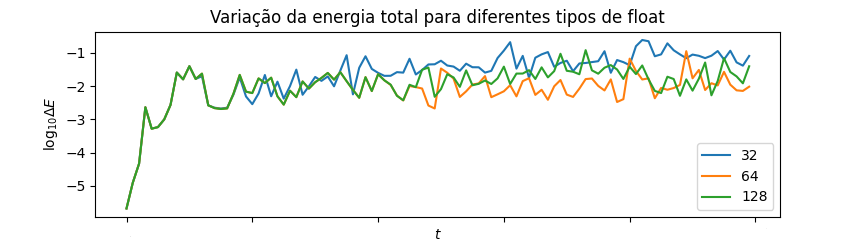
\includegraphics[width=\linewidth]{tcc//img/bits_energia.png}
    \caption{Variação da energia total no problema-modelo \ref{probmodelo:iau25} via método Ruth4 com $h=10^{-2}$ e $\epsilon=5h$ no intervalo $[0,500]$ para \textit{floats} com 32, 64 e 128 bits.}
    \label{fig:bits_energia}
\end{figure}

%%%%%%%%%%%%%%%%%%%%%%%%%%%%%%%%%%%%%
%%% PARALELIZAÇÃO
%%%%%%%%%%%%%%%%%%%%%%%%%%%%%%%%%%%%%
\subsection{Paralelização}\label{subsecao:paralelizacao}
Como mencionado anteriormente, foi utilizada uma biblioteca de Fortran para computação paralela, a \textit{OpenMP} (\textit{Open Multi-Processing}). Enquanto um código serial realiza uma operação por vez, um código paralelo é capaz de realizar mais de um cálculo ao mesmo tempo, como na figura \ref{fig:computacao_serial_paralela}. No caso do PCNG, existem algumas possibilidades para a aplicação: o cálculo do potencial e das forças, o cálculo da matriz normal utilizada no corretor numérico (ver equação (\ref{eq:corretor_matriz_normal})) e na detecção de colisões.

\begin{figure}[H]
    \centering
    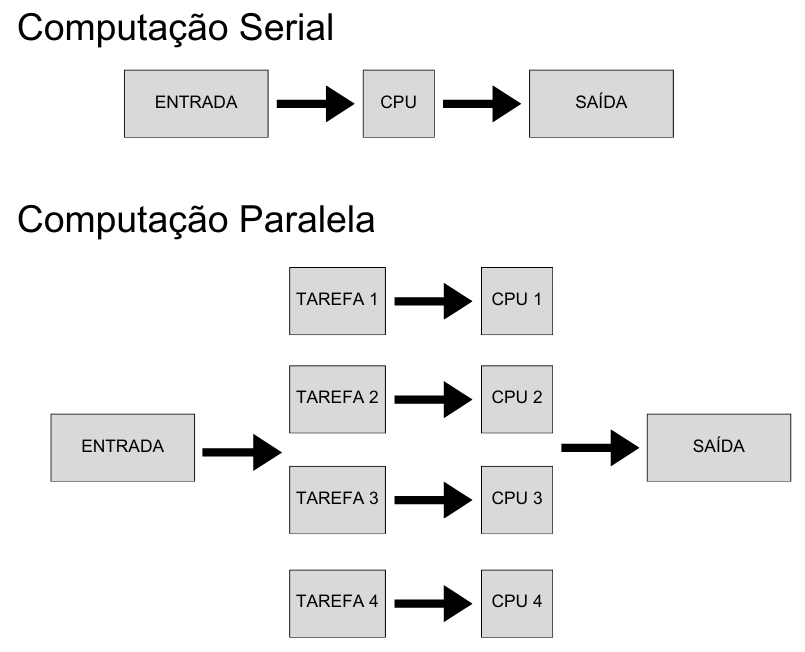
\includegraphics[width=0.5\linewidth]{tcc//img/computacao_serial_paralela.png}
        \caption{Visualização dos conceitos de computação serial e paralela.}
    \label{fig:computacao_serial_paralela}
\end{figure}

Exemplificando com o primeiro caso, foram implementadas duas funções de cálculo de forças: \verb|forcas_seq| e \verb|forcas_par|\footnote{O código completo consta em \cite{potalej_gravidade-fortran}.}. O núcleo do cálculo sequencial é feito da seguinte maneira:

\lstinputlisting[language=Fortran, caption=Código central da função sequencial de forças.]{tcc/codigos/forcas_seq.f90}

O valor \verb|distancia_inv| é o cubo do inverso da distância euclidiana entre os corpos, e \verb|Rab| é o vetor $\vet q_b - \vet q_a$. Observe como os \textit{loops} com \verb|DO| caracterizam a ordem quadrática dos cálculos. A proposta da paralelização neste caso está em dividir o cálculo da força para cada corpo entre os \textit{CPUs}, e posteriormente somar o resultado em um único vetor. Para isso, a biblioteca OpenMP permite definir variáveis compartilhadas (\verb|SHARED|, com as forças totais) e variáveis privadas (\verb|PRIVATE|, variáveis locais), o que garante que nenhuma CPU sobrescreva o vetor de forças das outras CPUs. A função paralelizada é semelhante à sequencial:

\lstinputlisting[language=Fortran, caption=Código central da função paralelizada de forças.]{tcc/codigos/forcas_par.f90}

Na figura \ref{fig:logtempo_paralelo_vs_sequencial} apresentamos um histograma em escala logarítmica com o tempo de computação (em segundos) para diferentes valores de $N$ com o método de Verlet e sem o uso de correção e de colisões, para garantir que o tempo esteja ligado diretamente com o cálculo das forças e do potencial. É possível observar que a diferença é expressiva para valores de $N$ a partir da centena, embora o cenário seja o oposto para valores de $N$ pequenos, uma vez que o custo de distribuir os cálculos entre os núcleos é maior que o do cálculo sequencial.

\begin{figure}
    \centering
    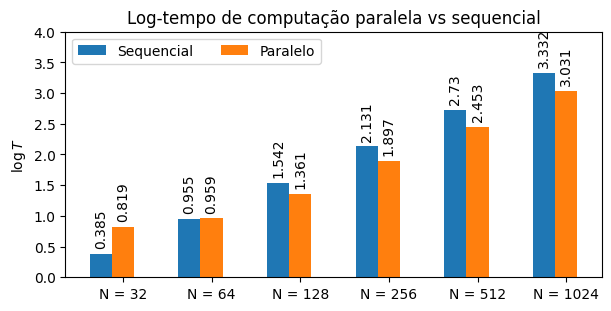
\includegraphics[width=0.8\linewidth]{tcc//img/logtempo.png}
    \caption{Log-tempo de computação paralela e computação sequencial para diferentes valores de $N$ e integração com método de Verlet, sem correção e sem colisão. Foram disponibilizados 4 núcleos para a paralelização.}
    \label{fig:logtempo_paralelo_vs_sequencial}
\end{figure}


%%%%%%%%%%%%%%%%%%%%%%%%%%%%%%%%%%%%%
%%% ARMAZENAMENTO
%%%%%%%%%%%%%%%%%%%%%%%%%%%%%%%%%%%%%
\subsection{Entrada e saída de dados}
Era objetivo que o programa final não contivesse somente simulações, mas facilitasse a geração de valores iniciais e a visualização dos dados também. Nesse sentido, há algumas opções disponíveis para a execução do programa, conforme tabela \ref{tabela:opcoes_entrada}.

\begin{table}
    \centering
    \begin{tabular}{c|c}
        \hline\hline
         \verb|-sv|, \verb|--sorteio-salvar|   & Sorteio de valores iniciais apenas \\
         \verb|-s|, \verb|--sorteio|           & Sorteio de valores iniciais e simulação \\
         \verb|-vi|, \verb|--valores-iniciais| & Simulação a partir de valores iniciais definidos \\
         \verb|-e|, \verb|--exibir|            & Exibição de trajetórias de uma simulação \\
         \verb|-d|, \verb|--dados|             & Exibição de dados de simulação \\
         \hline\hline
    \end{tabular}
    \caption{Opções de entrada no programa final.}
    \label{tabela:opcoes_entrada}
\end{table}

Existem também alguns tipos de arquivos diferentes utilizados pelo programa, os quais vale mencionar, conforme tabela \ref{tabela:arquivos_gerados}. Os arquivos do tipo 1 não são gerados, pois são o tipo mais simples, contendo informações como quantidade de corpos, valor das integrais primeiras, métodos \textit{etc}, sem definir valores iniciais explícitos.

\begin{table}
    \centering
    \begin{tabular}{c|c}
        \hline\hline
         1. & \textit{Preset} para sorteio \\
         2. & \textit{Preset} de valores iniciais \\
         3. & Informações de simulação (\textit{info.txt}) \\
         4. & Dados de simulação (\textit{data.csv}) \\
         \hline\hline
    \end{tabular}
    \caption{Arquivos utilizados ou gerados pelo programa.}
    \label{tabela:arquivos_gerados}
\end{table}

Os arquivos do tipo 1. podem ser usados para gerar valores iniciais explícitos através das chamadas \verb|-sv| e \verb|-s|, que têm entre as saídas um arquivo do tipo 2. Um exemplo de entrada consta no repositório do programa no diretório de \textit{presets}. Existem duas opções para a geração de valores iniciais: o sorteio \textit{comum} e o sorteio de \textit{Hénon}. No primeiro caso, apenas as integrais primeiras são condicionadas conforme o valor desejado. No segundo, são aplicadas as condições de Hénon, conforme descrito na seção \ref{secao:valores_iniciais}.

Já os arquivos de tipo 2 podem ser utilizados para as chamadas \verb|-vi|. Tais arquivos contêm configurações da simulação, como método, tamanho de passo e afins, e também os valores iniciais explícitos. O uso de tais arquivos facilita os testes com diferentes métodos para os mesmos valores iniciais.

Os arquivos de tipo 3 são gerados por simulações em ambas as chamadas \verb|-sv| e \verb|-vi|. Estes contêm informações acerca da simulação em si e de seu desempenho, podendo ser utilizados para comparações entre diferentes métodos. Por não ser um arquivo de entrada, é o que detém mais liberdade para conter diferentes informações. Um exemplo de arquivo de tipo 3 consta no programa \ref{prog:exemplo_saida}.

\lstinputlisting[label={prog:exemplo_saida}, caption={Exemplo de saída do arquivo de informações.}]{tcc/codigos/info.txt}

Por fim, os arquivos de tipo 4 contêm a constante $G$, o tamanho do passo, as massas, e as posições e momentos lineares no decorrer da simulação, armazenados no formato $(x, y, z, p_x, p_y, pz)$. Tais arquivos têm o formato \textit{.csv} (\textit{comma-separated values}). Esta não é a forma mais eficiente de armazenar dados do tipo, uma vez que a escrita de arquivos pelo Fortran é computacionalmente custosa e os arquivos ficam pesados. Para lidar com isso, existem tipos de arquivo mais eficientes, como o HDF\footnote{\textit{Hierarchical Data Format}. Para mais detalhes, veja: \href{https://www.hdfgroup.org/solutions/hdf5/}{https://www.hdfgroup.org/solutions/hdf5/}.}, mas por dificuldades técnicas e a facilidade de manipulação de CSV, a opção mais lenta foi escolhida.